% ============================================================================
%  Seção de metodologia — texto ORIGINAL do autor, com correção pontual apenas
%  dos dados que contradiziam o código do pacote bci_ortese.
%  A estrutura, a ordem dos parágrafos, os quadros, as equações e a redação
%  foram preservados. O que mudou está listado em CORRECOES_metodologia.md.
%
%  Este preâmbulo existe só para o arquivo compilar sozinho (pdflatex, 2x).
%  Para colar no TCC, use apenas o trecho entre INÍCIO e FIM DA SEÇÃO.
% ============================================================================
\documentclass[12pt,a4paper]{article}
\usepackage[T1]{fontenc}
\usepackage[utf8]{inputenc}
\IfFileExists{portuges.ldf}{\usepackage[brazil]{babel}}{\usepackage[english]{babel}}
\usepackage[margin=2.5cm]{geometry}
\usepackage{amsmath,amssymb}
\usepackage{graphicx}
\usepackage{array}
\usepackage{colortbl}
\usepackage{xcolor}
\usepackage{float}
\usepackage{caption}
\usepackage{hyperref}
\hypersetup{colorlinks=true,linkcolor=black,citecolor=black,urlcolor=blue}
\usepackage{helvet}
\renewcommand{\familydefault}{\sfdefault}
\linespread{1.5}
\graphicspath{{figuras/}}

\newcolumntype{L}[1]{>{\raggedright\arraybackslash}p{#1}}
\newcommand{\fonte}[1]{\par\vspace{2pt}{\footnotesize Fonte: #1}}
\newenvironment{quadro}[1][htbp]{\begin{table}[#1]}{\end{table}}
\captionsetup{font=small,labelfont=bf}
\newcommand{\citeonline}[1]{\cite{#1}}
\AtBeginDocument{%
  \renewcommand{\figurename}{Figura}%
  \renewcommand{\tablename}{Quadro}%
  \renewcommand{\refname}{Referências}%
}

\title{\vspace{-1.5cm}\large Materiais e métodos --- BCI de imagética motora para
acionamento de órtese\\[4pt]
\normalsize\normalfont Texto original com os dados corrigidos contra o código}
\author{}
\date{}

\begin{document}
\maketitle
\vspace{-1.2cm}

\section{Materiais e métodos}\label{sec:metodologia}

% ===================== INÍCIO DA SEÇÃO =====================

\subsection{Aquisição dos sinais EEG}\label{subsec:aquisicao}

A aquisição ao vivo é feita com um amplificador OpenBCI Cyton de oito canais e conversor de
24 bits, conectado ao computador por um \textit{dongle} serial e acessado pela biblioteca
BrainFlow. No \textit{dongle} USB a taxa de amostragem é fixa em 250\,Hz; as taxas superiores
previstas na placa exigem o módulo Wi-Fi, que não é utilizado.

Três eletrodos são empregados, posicionados segundo o sistema 10--20 sobre o córtex
sensório-motor: C3 no canal físico 1, C4 no canal 2 e Cz no canal 3. C3 e C4 formam o par
simétrico onde a lateralização do ERD se manifesta \cite{pfurtscheller1999}, e Cz serve de
referência central da linha média. A restrição a três eletrodos é deliberada, por viabilizar
uma montagem de baixo custo, e é também o principal limitante do desempenho, como discutido
na Seção~\ref{sec:resultados}.

O protocolo de captura implementado em \texttt{capturar.py} apresenta ao usuário, em tela
cheia, uma dica visual por segmento e grava a sessão inteira em fluxo contínuo, a 250\,Hz.
Cada execução contém 15 repetições de cada mão, sorteadas em ordem aleatória, com um
segmento de descanso de 4,1\,s antes de cada tarefa e 2\,s de estabilização do fluxo logo
após o início da transmissão. São 60 segmentos de 4,1\,s, cerca de 4,1 minutos de gravação.
Entre os segmentos não há pausa: eles são contíguos, porque as janelas de análise precisam de
metade do segmento anterior e qualquer intervalo não gravado cairia dentro delas. Foram
realizadas duas sessões, ambas de imagética e ambas com as três classes: mão direita, mão
esquerda e repouso. Antes de gravar, cada canal passa por remoção de tendência linear por
partes, com as quebras nos pontos médios entre eventos, e assim cada janela de análise
recebe a sua própria reta e o degrau entre retas cai na borda da janela, nunca no centro; as
demais etapas de filtragem ficam desligadas nesse ponto, porque a filtragem definitiva é
aplicada de forma idêntica a todas as fontes de dados na cadeia descrita a seguir. Cada
sessão é gravada em dois arquivos CSV, \texttt{continuo.csv} e \texttt{eventos.csv}, e o
código da classe fica na coluna \texttt{code} do segundo, de onde o rótulo é recuperado
posteriormente.

\subsection{Conjuntos de dados}\label{subsec:dados}

O treinamento combina duas origens. A principal é o \textit{PhysioNet EEG Motor
Movement/Imagery Dataset} \cite{eegmmidb2009}, adquirido com o sistema BCI2000
\cite{schalk2004}, do qual se utilizam 105 sujeitos e os seis \textit{runs} de mão: 3, 7 e
11, de movimento real, e 4, 8 e 12, de imagética. Os eventos anotados são T0 (repouso), T1
(mão esquerda) e T2 (mão direita), o que dá as três classes do problema. Essa seleção
percorre 630 arquivos e produz 18.266 janelas: a primeira anotação de cada \textit{run} é um
T0 no instante zero, sem segmento anterior para formar a metade esquerda da janela, e por
isso é descartada. A segunda origem são as gravações do próprio usuário, das quais se
aproveitam 87 janelas centradas; outras três caem pelo mesmo motivo. O pacote de distribuição
traz um subconjunto de dez sujeitos e duas sessões gravadas, suficiente para reproduzir a
cadeia e rodar um treino de demonstração, mas não para reconstruir o modelo completo.

Quatro sujeitos do conjunto público são descartados sempre. A auditoria dos arquivos mostrou
que o padrão é 160\,Hz, cerca de 123 a 125\,s e 30 eventos por \textit{run}, e que os
sujeitos S088 e S092 foram gravados a 128\,Hz com 38 eventos, o S100 a 128\,Hz com 24
eventos, e o \textit{run} R03 do S089 tem 181\,s e 44 eventos. A taxa divergente é o problema
mais grave, porque desalinha a duração das épocas. A exclusão reduz os 109 sujeitos do
eegmmidb aos 105 utilizados e é aplicada em um único ponto do código, para não se perder caso
a faixa de sujeitos seja ampliada.

O conjunto final tem 18.353 amostras, distribuídas em 8.860 de repouso, 4.773 de mão esquerda
e 4.720 de mão direita. O desbalanceamento é intrínseco ao protocolo do conjunto público: cada
tentativa de tarefa é seguida de um intervalo de repouso, de modo que a classe majoritária
tem aproximadamente o dobro de exemplos de cada classe motora.

\subsection{Cadeia de pré-processamento}\label{subsec:preproc}

A cadeia de pré-processamento obedece a uma restrição de projeto: ela é idêntica para os
arquivos EDF do conjunto público e para os CSV capturados ao vivo. Se
as duas fontes fossem tratadas de forma diferente, a rede seria treinada em um domínio e
operaria em outro. Por isso a cadeia está implementada no módulo \texttt{nucleo/preproc.py},
cuja função \texttt{cadeia\_mne()} é chamada tanto pela leitura de EDF quanto pela função
\texttt{janela\_bruta()}, que atende a leitura de janelas capturadas e a inferência em tempo
real. A Figura~\ref{fig:v9_preproc} mostra o efeito de cada etapa sobre uma gravação real.

\begin{figure}[htbp]
    \centering
    \caption{Cadeia de pré-processamento aplicada a uma gravação real do usuário. O trecho
    destacado em (d) é o preenchimento por reflexão discutido na
    Seção~\ref{subsubsec:janelas}.}
    \label{fig:v9_preproc}
    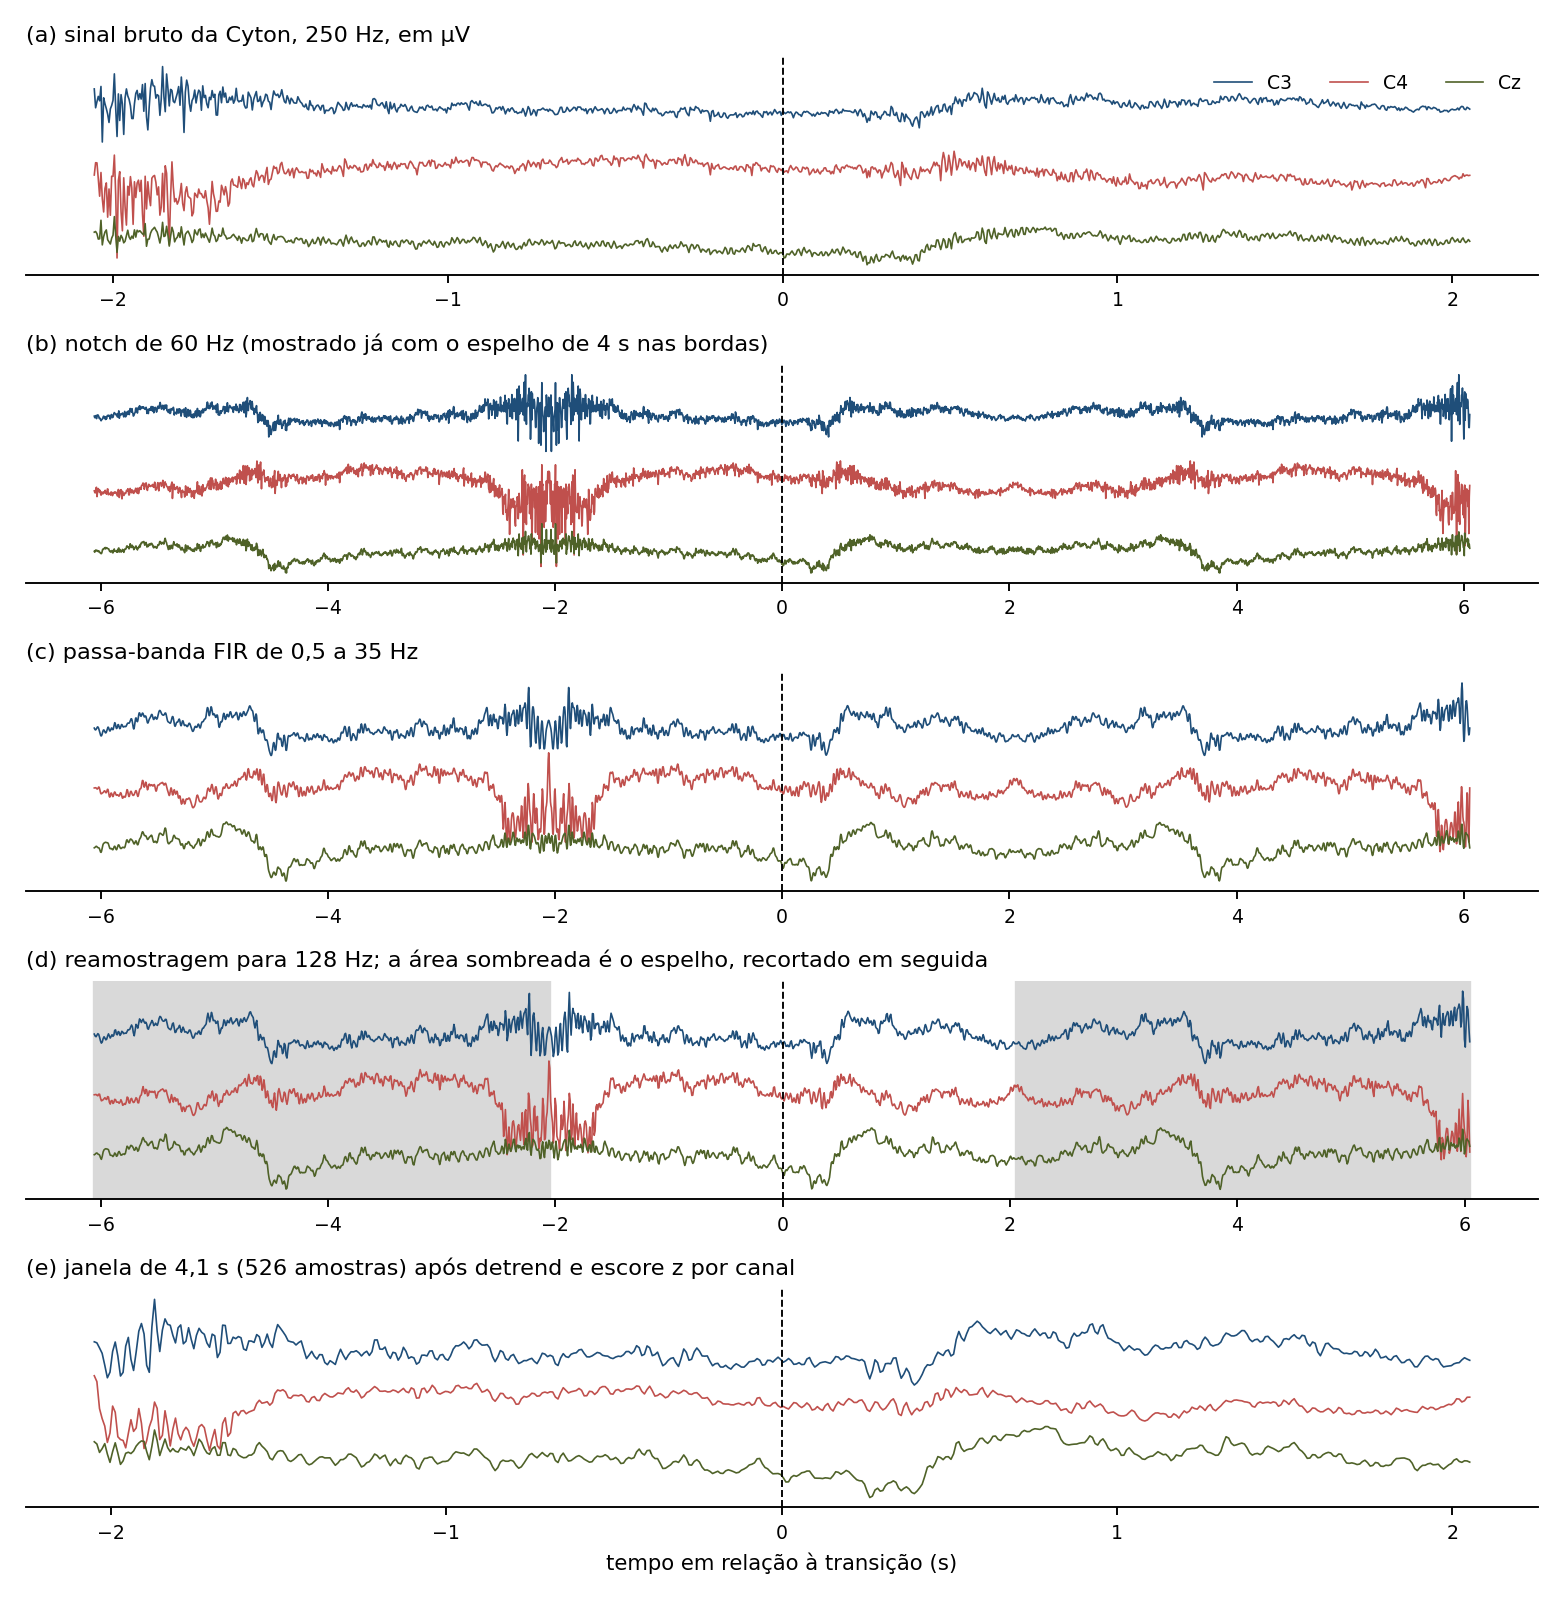
\includegraphics[width=0.86\textwidth]{v9_preprocessamento.png}
    \fonte{o autor (2026).}
\end{figure}

As etapas são: filtro \textit{notch} de 60\,Hz, para a interferência da rede elétrica;
passa-banda FIR de 0,5 a 35\,Hz, projetado por janelamento (\textit{firwin}); reamostragem
para 128\,Hz, taxa em que a rede opera e para a qual convergem os 250\,Hz da Cyton e os
160\,Hz do conjunto público; recorte da janela de $-2{,}05$\,s a $+2{,}05$\,s em torno da
transição entre segmentos, sem correção de linha de base em nenhuma das classes; remoção de
tendência linear; e normalização pelo escore $z$ por canal, conforme a
Equação~\ref{eq:zscore}, em que $\mu_c$ e $\sigma_c$ são a média e o desvio padrão do canal
$c$.

\begin{equation}\label{eq:zscore}
z_c[n] = \frac{x_c[n] - \mu_c}{\sigma_c}
\end{equation}

A normalização é o ponto em que treino e operação podem divergir sem que nada acuse a
diferença. A média e o desvio padrão são calculados apenas sobre o conjunto de treino e
gravados dentro do arquivo do modelo. Na inferência, a função
\texttt{normalizar\_com\_modelo()} recupera essas mesmas estatísticas do arquivo e as aplica
ao sinal novo, em vez de recalculá-las sobre o lote corrente. Assim, um sinal com amplitude
atípica não é reescalado para parecer normal, e a rede vê a mesma escala em que foi treinada.

\subsubsection{Remoção da referência média comum}

A versão anterior do sistema aplicava referência média comum (CAR) após selecionar C3, C4 e
Cz. Essa etapa foi removida das duas pontas da cadeia, e a razão é mensurável. Com apenas
três eletrodos, a CAR impõe $x_{\text{C3}} + x_{\text{C4}} + x_{\text{Cz}} = 0$ em cada
instante, e o posto da matriz de sinais cai de três para dois. A decomposição em valores
singulares de uma janela real mostrou, com a CAR aplicada, os dois primeiros valores
singulares na ordem de $4\times10^{-4}$ e o terceiro na ordem de $10^{-12}$; sem a CAR, o
terceiro valor volta à mesma ordem de grandeza dos demais. Oito ordens de grandeza abaixo dos
outros dois, o terceiro componente é numericamente nulo, e a rede recebia três canais com
apenas duas dimensões de informação.

A CAR só aproxima uma referência neutra quando há cobertura de toda a cabeça, o que uma
montagem de três eletrodos centrais não oferece. Aplicá-la apenas ao conjunto público, que
tem 64 canais, resolveria o problema numérico mas violaria a restrição de cadeia única, então
a etapa foi retirada dos dois lados.

\subsubsection{Tratamento das janelas curtas}\label{subsubsec:janelas}

As janelas de análise têm 4,1\,s a 128\,Hz e as duas origens chegam a esse comprimento por
caminhos diferentes. Duas correções são necessárias. A primeira é de borda: antes da
filtragem aplica-se preenchimento por reflexão de 4\,s em cada extremidade, porque o filtro
FIR de corte inferior em 0,5\,Hz precisa de contexto para não distorcer os extremos da
janela. Esse preenchimento é recortado logo após a filtragem, e o recorte é exato por
construção: qualquer que seja a taxa de origem, os 4\,s equivalem a
$4 \times 128 = 512$ amostras de cada lado depois da reamostragem, um número inteiro. Nenhuma
amostra espelhada nessa etapa chega à rede. A segunda correção é de comprimento:
$4{,}1 \times 128 = 524{,}8$ não é inteiro, e o projeto fixa 526 amostras contando as duas
pontas, enquanto o \texttt{mne.Epochs} devolve 525 para o EDF. A função
\texttt{ajustar\_tamanho()} completa o início por reflexão, mantendo intacto o fim da janela,
que contém a tarefa.

Medido sobre os arquivos do pacote, esse ajuste completa exatamente uma amostra por janela do
EDF, ou 0,19\,\% do comprimento, e nenhuma amostra nas gravações da Cyton e no laço de tempo
real, que chegam aos 526 pontos por conta própria. A mesma função recusa a janela com erro se
faltar mais de 2\,\% do comprimento, para que uma janela montada errado não passe
despercebida. O laço ao vivo solicita à placa a quantidade de amostras que corresponde à
janela completa do modelo, como descrito na Seção~\ref{subsec:online}, e por isso não há o
que completar. Uma versão anterior deste projeto gravava um arquivo por tentativa e deixava um
vão de cerca de 1,4\,s entre elas, e boa parte de cada janela de movimento tinha então de ser
fabricada por espelhamento; a gravação contínua eliminou esse problema.

\subsection{Construção das amostras}

Cada amostra é uma matriz de três linhas, na ordem C3, C4 e Cz, por 526 colunas,
correspondentes a 4,1\,s amostrados a 128\,Hz. O rótulo vem da anotação do evento, no caso
dos arquivos públicos, ou do código registrado em \texttt{eventos.csv}, no caso das gravações
próprias, segundo o mapeamento \texttt{RE}~$\rightarrow$~repouso,
\texttt{LH}~$\rightarrow$~esquerda e \texttt{RH}~$\rightarrow$~direita. O tensor entregue à
rede tem forma $(N, 3, 526)$ e recebe uma dimensão de canal unitário internamente, passando a
$(N, 1, 3, 526)$, de modo que as convoluções bidimensionais tratem o eixo dos eletrodos e o
eixo do tempo separadamente.

\subsection{Arquitetura da rede}\label{subsec:arquitetura}

O classificador opera diretamente sobre a forma de onda, sem extração manual de
características. A Figura~\ref{fig:v9_arq} mostra a sequência de camadas com as formas dos
tensores lidas do próprio modelo, e o Quadro~\ref{qua:camadas} detalha cada operação com seus
parâmetros.

\begin{figure}[htbp]
    \centering
    \caption{Camadas da rede e formas dos tensores em cada estágio.}
    \label{fig:v9_arq}
    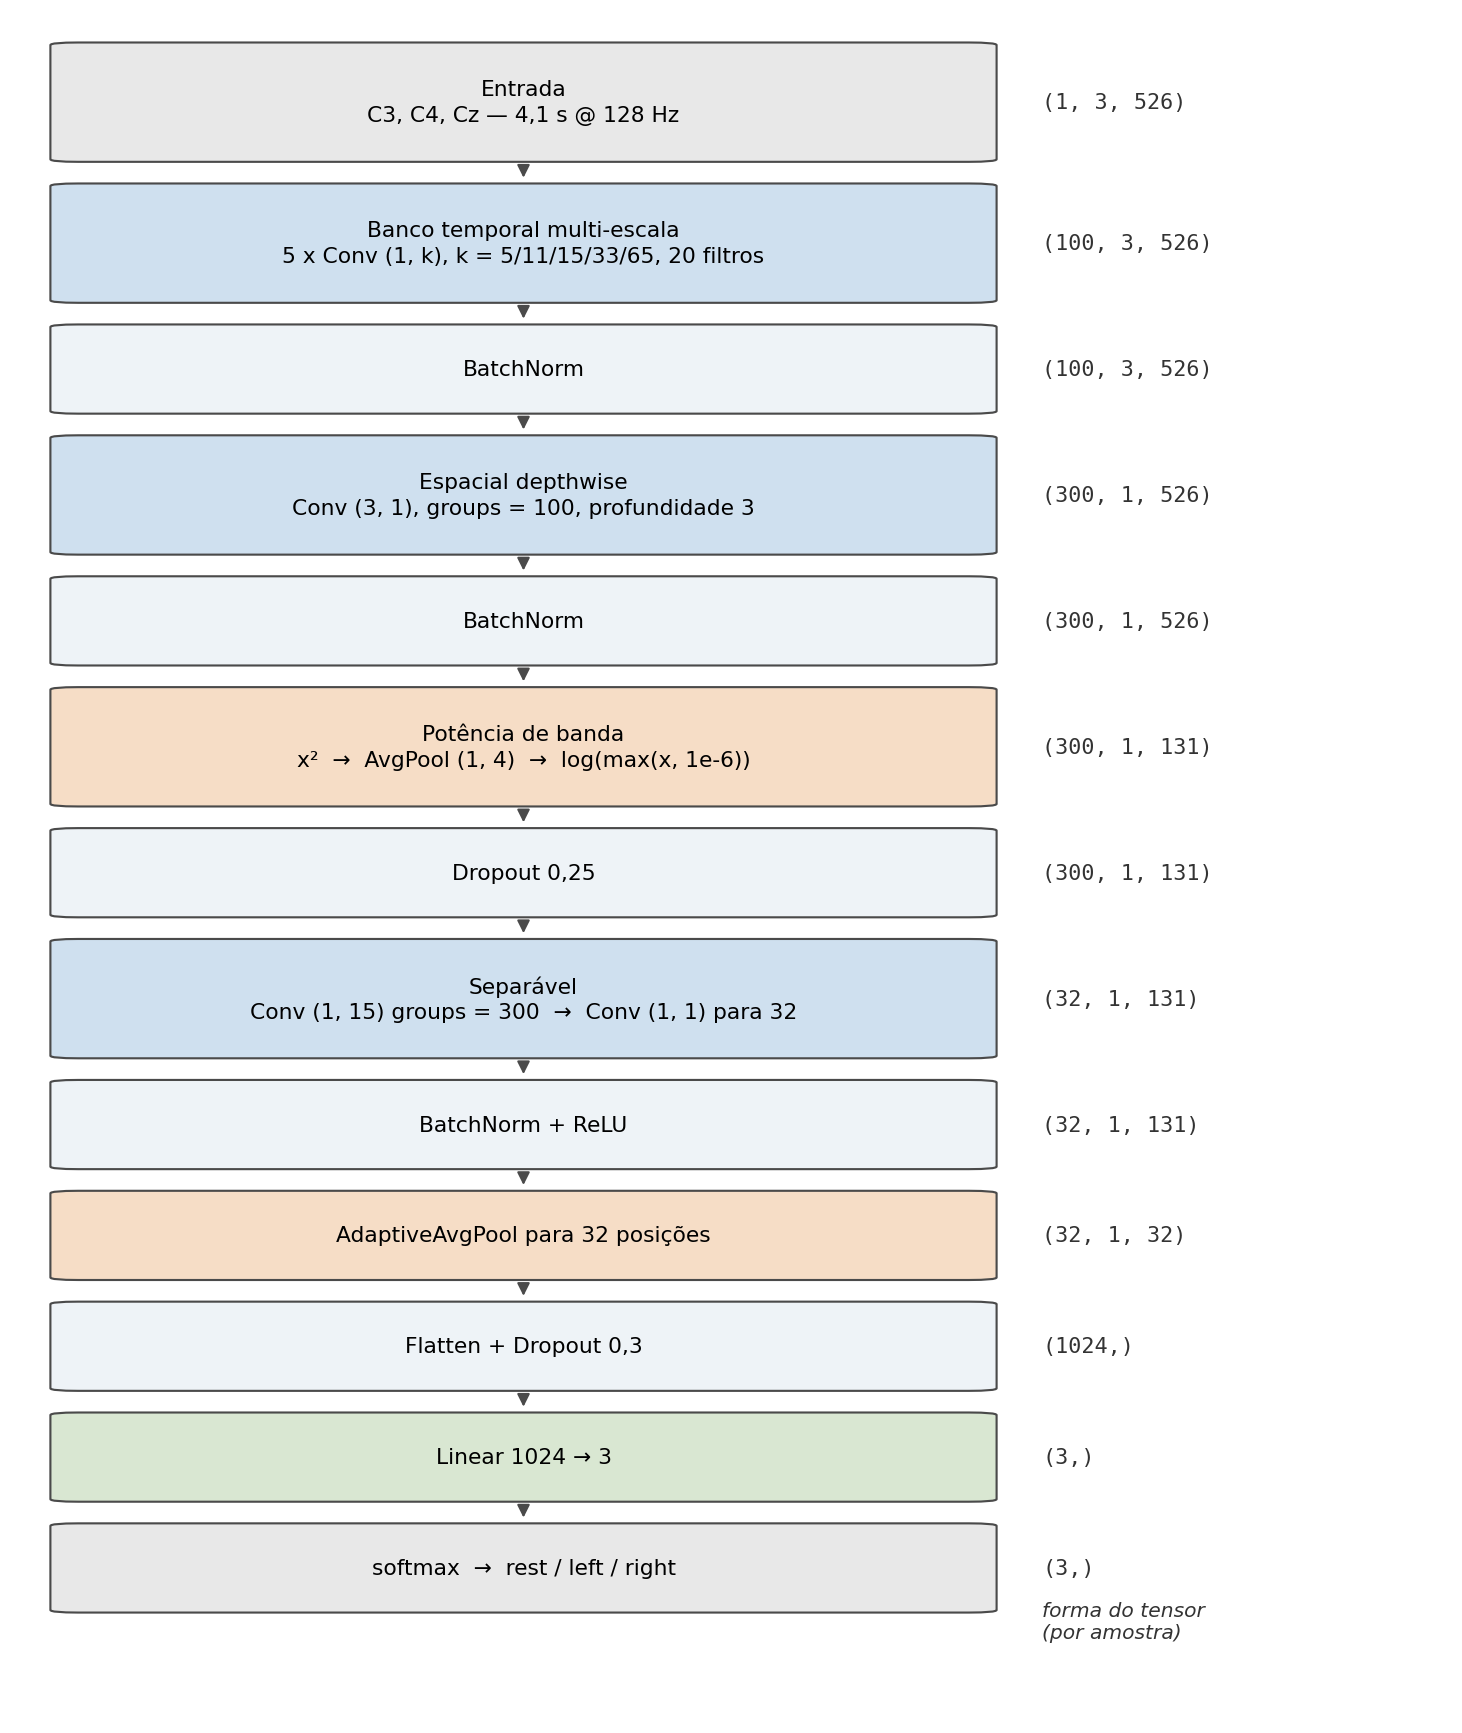
\includegraphics[width=0.55\textwidth]{v9_arquitetura.png}
    \fonte{o autor (2026).}
\end{figure}

\begin{quadro}[htbp]
\centering
\caption{Arquitetura da CNN, camada a camada. Formas de saída por amostra, sem a dimensão de
lote.}
\label{qua:camadas}
\footnotesize
\renewcommand{\arraystretch}{1.12}
\begin{tabular}{|c|L{4.5cm}|L{4.4cm}|r|l|}
\hline
\rowcolor[HTML]{EFEFEF}
\textbf{\#} & \textbf{Camada} & \textbf{Operação} & \textbf{Param.} & \textbf{Saída} \\ \hline
0 & Entrada & C3, C4 e Cz, 4,1\,s a 128\,Hz & 0 & $(1, 3, 526)$ \\ \hline
1 & Banco temporal multi-escala & 5 convoluções paralelas $(1{,}k)$, $k \in \{5, 11, 15, 33, 65\}$, 20 filtros cada, preenchimento $k/2$, sem viés & 2.580 & $(100, 3, 526)$ \\ \hline
2 & Normalização em lote & \textit{BatchNorm} sobre 100 mapas & 200 & $(100, 3, 526)$ \\ \hline
3 & Espacial \textit{depthwise} & convolução $(3{,}1)$ com \textit{groups}~=~100 e profundidade 3, sem viés & 900 & $(300, 1, 526)$ \\ \hline
4 & Normalização em lote & \textit{BatchNorm} sobre 300 mapas & 600 & $(300, 1, 526)$ \\ \hline
5 & Quadrado & $x^{2}$, elemento a elemento & 0 & $(300, 1, 526)$ \\ \hline
6 & Média móvel & \textit{average pooling} $(1{,}4)$ & 0 & $(300, 1, 131)$ \\ \hline
7 & Logaritmo com piso & $\log(\max(x, 10^{-6}))$ & 0 & $(300, 1, 131)$ \\ \hline
8 & \textit{Dropout} 0,25 & regularização & 0 & $(300, 1, 131)$ \\ \hline
9 & Separável (temporal) & convolução $(1{,}15)$ com \textit{groups}~=~300, preenchimento 7, sem viés & 4.500 & $(300, 1, 131)$ \\ \hline
10 & Separável (pontual) & convolução $(1{,}1)$ de 300 para 32 mapas, sem viés & 9.600 & $(32, 1, 131)$ \\ \hline
11 & Normalização em lote e ReLU & \textit{BatchNorm} e retificação & 64 & $(32, 1, 131)$ \\ \hline
12 & \textit{Pooling} adaptativo & média para 32 posições temporais & 0 & $(32, 1, 32)$ \\ \hline
13 & Achatamento e \textit{dropout} 0,3 & vetor de características & 0 & $(1024,)$ \\ \hline
14 & Camada linear & projeção para as três classes & 3.075 & $(3,)$ \\ \hline
\rowcolor[HTML]{EFEFEF}
\multicolumn{3}{|r|}{\textbf{Total de parâmetros treináveis}} & \textbf{21.519} & \\ \hline
\end{tabular}
\fonte{o autor (2026), a partir de \texttt{nucleo/modelo.py} e \texttt{config.py}.}
\end{quadro}

\subsubsection{Banco temporal multi-escala}

A primeira camada é um banco de filtros aprendidos, organizado em cinco escalas paralelas de
20 filtros cada. Cada filtro percorre o eixo do tempo de um eletrodo por vez, sem misturar
eletrodos. Para um kernel $w$ de comprimento $k$ aplicado ao canal $c$, a saída no instante
$n$ é dada pela Equação~\ref{eq:conv_temporal}:

\begin{equation}\label{eq:conv_temporal}
h_{f}[c, n] = \sum_{j=0}^{k-1} w_{f}[j]\, x\!\left[c,\, n + j - \left\lfloor k/2 \right\rfloor \right],
\end{equation}

\noindent em que o deslocamento $\lfloor k/2 \rfloor$ decorre do preenchimento simétrico, que
preserva o comprimento da janela. Os cinco ramos são concatenados no eixo de mapas,
produzindo 100 mapas temporais.

O motivo de usar escalas diferentes está na relação entre o comprimento do kernel e a
frequência que ele consegue representar, e essa relação é frequentemente lida ao contrário. O
comprimento limita a frequência mais \emph{baixa} representável, não a mais alta: um ciclo
inteiro precisa caber dentro do kernel. A 128\,Hz, um kernel de comprimento $k$ representa a
partir de $128/k$\,Hz, de modo que são os ramos curtos que alcançam o teto de 35\,Hz da
banda. O painel (a) da Figura~\ref{fig:v9_kernels} mostra a faixa coberta por cada escala e o
painel (b), a resposta em frequência média dos filtros aprendidos, extraída dos
pesos do modelo treinado.

\begin{figure}[htbp]
    \centering
    \caption{Banco de filtros multi-escala: faixa representável por escala e resposta em
    frequência dos filtros aprendidos.}
    \label{fig:v9_kernels}
    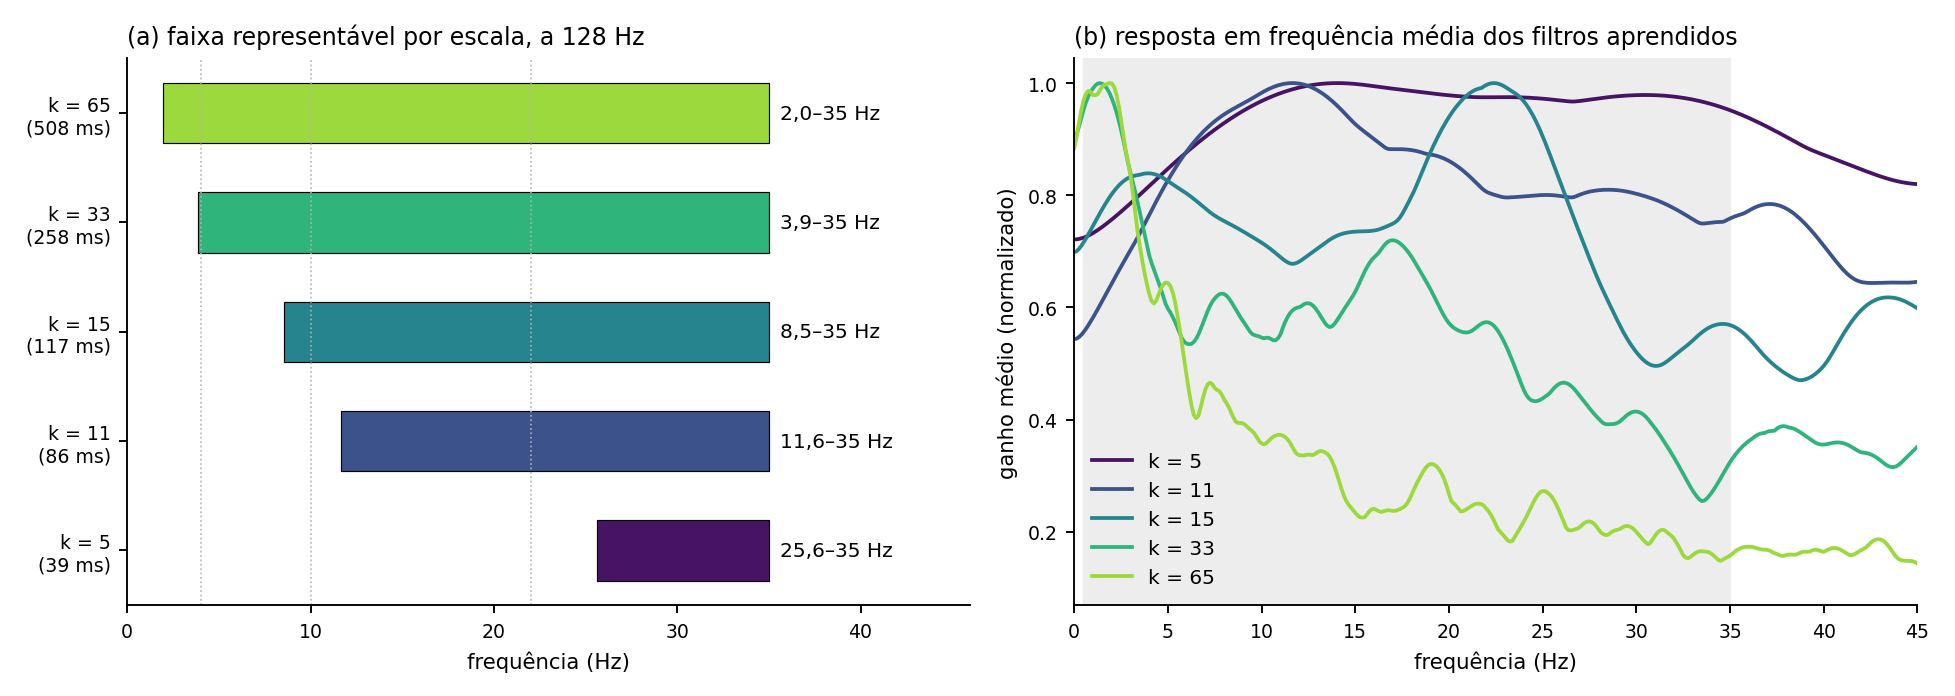
\includegraphics[width=0.94\textwidth]{v9_kernels.png}
    \fonte{o autor (2026).}
\end{figure}

O Quadro~\ref{qua:escalas} relaciona cada escala ao seu limite inferior. O ramo mais longo, de
65 amostras, alcança 2,0\,Hz e cobre a faixa lenta em que se manifestam os potenciais
corticais relacionados a movimento; o mais curto, de 5 amostras, cobre a porção alta de
$\beta$.

\begin{quadro}[htbp]
\centering
\caption{Escalas temporais do banco de filtros e faixa de frequência que cada uma consegue
representar a 128\,Hz.}
\label{qua:escalas}
\footnotesize
\begin{tabular}{|c|c|c|c|l|}
\hline
\rowcolor[HTML]{EFEFEF}
\textbf{Escala} & \textbf{Comprimento} & \textbf{Duração} & \textbf{Representa a partir de} & \textbf{Faixa} \\ \hline
1 & 5  & 39\,ms  & 25,6\,Hz & $\beta$ alto \\ \hline
2 & 11 & 86\,ms  & 11,6\,Hz & $\beta$ \\ \hline
3 & 15 & 117\,ms & 8,5\,Hz  & $\mu$ / $\alpha$ \\ \hline
4 & 33 & 258\,ms & 3,9\,Hz  & $\theta$ \\ \hline
5 & 65 & 508\,ms & 2,0\,Hz  & $\delta$ e potenciais lentos \\ \hline
\end{tabular}
\fonte{o autor (2026).}
\end{quadro}

\subsubsection{Filtro espacial \textit{depthwise}}

A segunda camada colapsa os três eletrodos em uma única linha, mas de forma agrupada: cada um
dos 100 mapas temporais recebe seus próprios três filtros espaciais, em vez de uma convolução
densa que misturasse todas as escalas. Para o mapa $f$ e o filtro espacial $d$, a operação é a
combinação linear dos eletrodos dada pela Equação~\ref{eq:conv_espacial}:

\begin{equation}\label{eq:conv_espacial}
z_{f,d}[n] = \sum_{c=1}^{3} v_{f,d}[c]\, \hat{h}_{f}[c, n],
\end{equation}

\noindent em que $\hat{h}_f$ é o mapa temporal já normalizado. O agrupamento permite que cada
faixa de frequência aprenda sua própria topografia, o que é razoável porque não há motivo
para o ERD em $\mu$ e o ERD em $\beta$ apresentarem a mesma distribuição entre C3 e C4.
Trata-se do análogo aprendido de um filtro espacial do tipo CSP \cite{ramoser2000,ang2008}. A
profundidade 3 é o teto útil da montagem: com três eletrodos não existem mais de três
direções espaciais independentes. O resultado são 300 mapas de uma linha por 526 colunas.

\subsubsection{Camada de potência}

O bloco seguinte converte amplitude em potência de banda, e é a principal decisão de projeto
da arquitetura. Após a convolução
espacial, o sinal é elevado ao quadrado, submetido a uma média móvel de quatro amostras e
passado por um logaritmo, conforme a Equação~\ref{eq:potencia}:

\begin{equation}\label{eq:potencia}
p_{f,d}[m] = \log\!\left( \max\!\left( \frac{1}{4} \sum_{n=4m}^{4m+3} z_{f,d}[n]^{2},\; \varepsilon \right) \right), \qquad \varepsilon = 10^{-6}.
\end{equation}

Essa composição é a log-variância empregada no FBCSP \cite{ang2008}, isto é, a potência de
banda em janelas curtas, a grandeza física em que o ERD e o ERS são definidos
\cite{pfurtscheller1999}. O mesmo bloco aparece na ShallowFBCSPNet de
\citeonline{schirrmeister2017}, projetada com essa motivação. O piso $\varepsilon$ evita que
potências próximas de zero produzam $-\infty$ e anulem o gradiente.

Não há função de ativação retificadora antes do quadrado, e isso é deliberado: o quadrado
\emph{é} a não-linearidade da cadeia. Retificar antes destruiria a medida de potência, porque
a ReLU descarta o semiciclo negativo de uma oscilação e a média de um sinal oscilatório tende
a zero. A versão anterior do classificador usava retificação seguida de \textit{max pooling}
nesse ponto, combinação inadequada para sinal oscilatório e substituída pelo bloco de potência
pelo motivo apontado por \citeonline{schirrmeister2017}.

\subsubsection{Bloco separável e classificação}

O último bloco convolucional é uma convolução separável, no padrão do segundo bloco da EEGNet
\cite{lawhern2018}: primeiro uma convolução temporal de comprimento 15 aplicada a cada mapa
isoladamente, que refina o eixo do tempo sem misturar mapas, e depois uma convolução pontual
$1\times1$ que reduz os 300 mapas a 32. Seguem normalização em lote, retificação e um
\textit{pooling} adaptativo que fixa a saída em 32 posições temporais, tornando a rede
independente do comprimento exato da janela. O vetor achatado de 1.024 elementos passa por
\textit{dropout} de 0,3 e por uma camada linear que produz os três \textit{logits}. A
conversão em probabilidades é feita pela função \textit{softmax}, Equação~\ref{eq:softmax}:

\begin{equation}\label{eq:softmax}
P(y = i \mid x) = \frac{e^{\,o_i}}{\sum_{j=1}^{3} e^{\,o_j}}, \qquad i \in \{\text{rest}, \text{left}, \text{right}\},
\end{equation}

\noindent em que $o_i$ é o \textit{logit} da classe $i$. A classe predita é a de maior
probabilidade, e o vetor completo de probabilidades é o que alimenta a regra de decisão
descrita na Seção~\ref{subsec:online}.

\subsection{O que as convoluções extraem do sinal}

Os filtros não representam os conceitos ``mão esquerda'' ou ``mão direita''. O que se ajusta
durante o treinamento são pesos que maximizam a separabilidade das três classes segundo a
função de perda; o resultado é um conjunto de projeções temporais e espaciais cujas
combinações discriminam as classes no conjunto de treino. A camada temporal aprende respostas
em frequência: o painel (b) da Figura~\ref{fig:v9_kernels} mostra que os ramos de kernel longo
concentram ganho na porção baixa do espectro e os de kernel curto se espalham até o teto da
banda, comportamento coerente com o limite $128/k$. A camada espacial, por sua vez, aprende
pesos relativos entre C3, C4 e Cz por faixa. A camada de potência converte essas projeções na
grandeza em que o ERD é definido.

Isso não equivale a afirmar que um filtro específico corresponde a um fenômeno fisiológico
determinado. A resposta em frequência exibida é uma visualização dos pesos treinados, não uma
identificação de gerador cortical. A leitura fisiológica que o projeto sustenta é a de nível
de sistema: a arquitetura foi construída para medir potência de banda por eletrodo e por
faixa, que é onde a literatura localiza a assinatura da imagética motora
\cite{pfurtscheller1999,pfurtscheller2001}.

\subsection{Treinamento}\label{subsec:treinamento}

O modelo é treinado do zero, sem partir de pesos anteriores. Os checkpoints da versão anterior
do projeto pertencem a outra arquitetura, de kernel único e retificação com \textit{max
pooling}, e a uma cadeia de pré-processamento que incluía a CAR; reaproveitá-los transferiria
pesos ajustados a uma representação diferente. O Quadro~\ref{qua:treino} reúne os
hiperparâmetros.

\begin{quadro}[htbp]
\centering
\caption{Hiperparâmetros de treinamento.}
\label{qua:treino}
\footnotesize
\renewcommand{\arraystretch}{1.12}
\begin{tabular}{|L{4.6cm}|L{9.0cm}|}
\hline
\rowcolor[HTML]{EFEFEF}
\textbf{Parâmetro} & \textbf{Valor} \\ \hline
Inicialização & aleatória (sem \textit{checkpoint} anterior) \\ \hline
Épocas & 35 \\ \hline
Tamanho do lote & 16 no treino; 64 na validação, apenas para limitar o pico de memória \\ \hline
Otimizador & Adam, taxa de aprendizado $10^{-3}$ \\ \hline
Função de perda & entropia cruzada com pesos por classe, proporcionais ao inverso da frequência \\ \hline
Divisão treino/validação & 80\,\%/20\,\%, estratificada por classe e por origem do dado: 14.683 e 3.670 janelas \\ \hline
Sementes & 40 nos geradores do PyTorch, do Python e do NumPy \\ \hline
Aumento de dados & escala de amplitude entre 0,9 e 1,1; deslocamento temporal de até $\pm16$ amostras; ruído gaussiano de desvio 0,10, cada um com probabilidade 0,5, apenas no conjunto de treino \\ \hline
Repetição das gravações próprias & fator 8 no conjunto de treino: 490 janelas acrescentadas, levando o treino a 15.173 \\ \hline
Seleção do modelo & melhor acurácia de validação ao longo das épocas (época 15, no treino do modelo distribuído) \\ \hline
Processamento & CPU \\ \hline
\end{tabular}
\fonte{o autor (2026), a partir de \texttt{config.py}.}
\end{quadro}

A perda ponderada, Equação~\ref{eq:ce}, compensa o desbalanceamento das classes descrito na
Seção~\ref{subsec:dados}:

\begin{equation}\label{eq:ce}
\mathcal{L} = -\frac{1}{N}\sum_{i=1}^{N} \alpha_{y_i} \log P(y_i \mid x_i), \qquad \alpha_{c} \propto \frac{1}{n_c},
\end{equation}

\noindent em que $n_c$ é o número de amostras da classe $c$ e os pesos $\alpha_c$ são
normalizados para somar o número de classes.

O aumento de dados aplicado durante o treinamento é o conjunto de três
transformações listado no Quadro~\ref{qua:treino}, sorteadas de forma independente a cada
apresentação da amostra e restritas ao conjunto de treino.

O aumento de dados sorteia suas transformações com o módulo \texttt{random} do Python, e não
com o gerador do PyTorch. Semear apenas o PyTorch, portanto, deixava duas execuções
nominalmente idênticas divergirem, e por isso os três geradores são semeados no início do
treino. A repetição das gravações próprias por um fator 8 responde a uma segunda dificuldade:
elas são 87 das 18.353 janelas, menos de 0,5\,\% do conjunto, e desapareceriam no lote sem
esse reforço. A repetição incide apenas sobre as 70 que caíram no treino, e nenhuma janela
repetida entra na validação. A ressalva correspondente está na Seção~\ref{sec:resultados}.

A divisão em treino e validação é estratificada simultaneamente por classe e por origem, o que
permite reportar a acurácia separadamente para o conjunto público e para as gravações
próprias. As estatísticas de normalização são calculadas apenas sobre as amostras de treino,
depois de definida a divisão, e gravadas no arquivo do modelo junto com os pesos e com a
descrição da arquitetura. Esse último campo permite que o arquivo reconstrua a rede exatamente
como foi treinada, mesmo que os valores padrão da classe mudem posteriormente.

\subsection{Inferência sobre arquivos gravados}

O comando \texttt{inferir\_offline.py} carrega o modelo, reaplica a cadeia de pré-processamento
e classifica os arquivos indicados. Aceita tanto os EDF do conjunto público, caso em que
reconstrói as épocas a partir das anotações e compara com o rótulo verdadeiro, quanto os CSV
capturados, caso em que recupera o rótulo do arquivo de eventos. A saída traz, por janela, a
probabilidade de cada classe e a decisão, além da acurácia agregada e da matriz de confusão
quando há rótulo disponível. Nas gravações contínuas o programa faz ainda uma segunda leitura,
por janela deslizante, que varre o sinal inteiro sem usar os eventos e mede quantos comandos a
órtese receberia. É o modo usado para avaliar o modelo e para produzir os números da
Seção~\ref{sec:resultados}.

\subsection{Inferência em tempo real com o capacete}\label{subsec:online}

A operação ao vivo é implementada em \texttt{tempo\_real.py} e executa um laço com passo de
0,25\,s. A cada iteração o programa solicita à placa as últimas 1.028 amostras, que a 250\,Hz
correspondem a 4,11\,s, a janela que o modelo enxerga após a reamostragem para
128\,Hz. Essa quantidade é calculada a partir do comprimento de janela lido do próprio arquivo
do modelo, e não de um número fixo; com isso o \textit{buffer} acompanha automaticamente
qualquer mudança de janela ou de taxa.

O bloco lido passa pela mesma função usada para as gravações, que aplica o espelho nas bordas,
a filtragem, a reamostragem e a remoção de tendência linear por canal. A normalização usa as
estatísticas gravadas no modelo. A rede produz o vetor de probabilidades e a decisão é tomada
pela regra da Equação~\ref{eq:regra}:

\begin{equation}\label{eq:regra}
\hat{y} =
\begin{cases}
\text{left}, & \text{se } P(\text{left} \mid x) > 0{,}50 \\[2pt]
\text{right}, & \text{se } P(\text{right} \mid x) > 0{,}50 \text{ e } P(\text{left} \mid x) \leq 0{,}50 \\[2pt]
\text{rest}, & \text{caso contrário.}
\end{cases}
\end{equation}

Entre o rótulo da janela isolada e o comando enviado à órtese está a classe
\texttt{Decisor}, que trava o estado por 3,0\,s depois de mandar fechar e impõe 2,0\,s de tempo
morto antes de um novo acionamento. A trava é necessária porque a evidência que a rede usa é o
transiente da transição, que sai da janela deslizante poucos segundos depois do início do
movimento; exigir confirmação contínua faria a mão reabrir sozinha enquanto o usuário ainda
tenta fechá-la.

O limiar existe para conter disparos falsos, que numa órtese significam a mão fechando
sozinha. A varredura por
janela deslizante em seis \textit{runs} contínuos do PhysioNet (44 tentativas, 740\,s, passo de
0,25\,s) produziu a relação registrada no \texttt{config.py}: com limiar 0,60, 73\,\% de
detecção e um disparo falso a cada 16\,s; com 0,70, 68\,\% e um a cada 29\,s; com 0,80, 43\,\%
e um a cada 53\,s. Há uma divergência interna no pacote: essa tabela e os
comentários do código apontam 0,80 como escolha, mas o valor atribuído a
\texttt{config.LIMIAR} é 0,50, que é o que os programas usam enquanto a linha não for alterada.

O percurso de treino e o de operação diferem em poucos pontos: a origem do sinal, arquivo em um
caso e transmissão contínua da placa no outro; o comprimento solicitado, ajustado ao modelo na
operação ao vivo; e a decisão, que no treino é o simples máximo das probabilidades e na
operação passa pelo limiar e pela trava. A filtragem, a reamostragem, o recorte, a remoção de
tendência e a normalização são executados pelo mesmo código nos dois casos.

Para verificação sem o hardware de atuação, \texttt{tempo\_real.py} com a opção
\texttt{-{}-sem-ortese} executa o mesmo laço sem abrir a porta serial, imprimindo apenas as
probabilidades e a decisão; com \texttt{-{}-simular-ortese}, imprime também os comandos que
seriam enviados.

\subsection{Integração com a órtese}

Quando a decisão coincide com a classe configurada como alvo, o programa envia bytes pela porta
serial a 115200\,baud. O \textit{firmware} do ESP32 mantém um laço de leitura da serial e
interpreta quatro comandos, de um byte cada e sem terminador: \texttt{R} incrementa o ângulo
até o teto de 180$^{\circ}$, \texttt{L} decrementa até $-30^{\circ}$, \texttt{C} leva o servo a
90$^{\circ}$, que é o centro do curso e a posição de repouso da órtese, e um dígito de
\texttt{0} a \texttt{9} define o tamanho do passo em graus. A cada byte recebido o firmware
imprime \texttt{angle=<n>}, e o lado do PC lê esse eco e o usa como posição real, em vez de
contar pulsos às cegas. O servomotor é acionado no GPIO~18, configurado a 50\,Hz com largura de
pulso entre 500 e 2500\,\textmu s. O deslocamento entre o ângulo de repouso, 90$^{\circ}$, e o
de mão fechada, 120$^{\circ}$, é executado em passos de 3$^{\circ}$ a cada 50\,ms, portanto dez
pulsos, e não de uma vez: o movimento gradual evita o golpe abrupto sobre a estrutura impressa
e reduz o pico de corrente do atuador. Como o firmware não limita o curso à amplitude da
órtese, essa limitação fica no PC, que recorta qualquer alvo ao intervalo entre repouso e fechado e
devolve a órtese ao repouso ao encerrar.

Um segundo modo de acionamento, disponível em \texttt{inferir\_offline.py} com a opção
\texttt{-{}-ortese}, classifica uma gravação já existente e aciona o microcontrolador durante a
varredura, aplicando o mesmo limiar de probabilidade. Esse modo serve à demonstração
controlada do encadeamento completo, com rótulo conhecido, e a opção
\texttt{-{}-simular-ortese} imprime os comandos que seriam enviados sem abrir a porta serial.

% ===================== FIM DA SEÇÃO =====================

% Âncora apenas para este arquivo compilar sozinho. No TCC completo, apague as duas
% linhas abaixo: a seção de resultados já define este rótulo.
\phantomsection
\label{sec:resultados}

\begin{thebibliography}{9}
\bibitem{ang2008} ANG, K. K. \textit{et al.} Filter Bank Common Spatial Pattern (FBCSP) in
brain-computer interface. \textbf{IEEE International Joint Conference on Neural Networks},
p. 2390--2397, 2008.
\bibitem{eegmmidb2009} GOLDBERGER, A. L. \textit{et al.} PhysioBank, PhysioToolkit, and
PhysioNet: components of a new research resource for complex physiologic signals.
\textbf{Circulation}, v. 101, n. 23, p. e215--e220, 2000.
\bibitem{lawhern2018} LAWHERN, V. J. \textit{et al.} EEGNet: a compact convolutional neural
network for EEG-based brain-computer interfaces. \textbf{Journal of Neural Engineering},
v. 15, n. 5, 056013, 2018.
\bibitem{pfurtscheller1999} PFURTSCHELLER, G.; LOPES DA SILVA, F. H. Event-related EEG/MEG
synchronization and desynchronization: basic principles. \textbf{Clinical Neurophysiology},
v. 110, n. 11, p. 1842--1857, 1999.
\bibitem{pfurtscheller2001} PFURTSCHELLER, G.; NEUPER, C. Motor imagery and direct
brain-computer communication. \textbf{Proceedings of the IEEE}, v. 89, n. 7, p. 1123--1134,
2001.
\bibitem{ramoser2000} RAMOSER, H.; MÜLLER-GERKING, J.; PFURTSCHELLER, G. Optimal spatial
filtering of single trial EEG during imagined hand movement. \textbf{IEEE Transactions on
Rehabilitation Engineering}, v. 8, n. 4, p. 441--446, 2000.
\bibitem{schalk2004} SCHALK, G. \textit{et al.} BCI2000: a general-purpose brain-computer
interface (BCI) system. \textbf{IEEE Transactions on Biomedical Engineering}, v. 51, n. 6,
p. 1034--1043, 2004.
\bibitem{schirrmeister2017} SCHIRRMEISTER, R. T. \textit{et al.} Deep learning with
convolutional neural networks for EEG decoding and visualization. \textbf{Human Brain
Mapping}, v. 38, n. 11, p. 5391--5420, 2017.
\end{thebibliography}

\end{document}
